% Copyright (C) 2007 Thomas L. Kula
% All Rights Reserved
%
% See the file LICENSE for license terms.
\documentclass[12pt]{article}
\usepackage{graphicx}
\setlength{\paperwidth}{5.5in}
\setlength{\paperheight}{8.5in}
\setlength{\textheight}{7.45in}
\setlength{\topmargin}{-1.0in}
\setlength{\oddsidemargin}{-0.5in}
\setlength{\evensidemargin}{-0.5in}
\setlength{\textwidth}{4.0in}
\setlength{\parindent}{0in}
\setlength{\parskip}{3mm}
\usepackage[print]{booklet} \nofiles
\source{\magstep0}{5.5in}{8.5in}
\target{\magstep0}{11in}{8.5in}
\setpdftargetpages
\pagestyle{empty}
\begin{document}



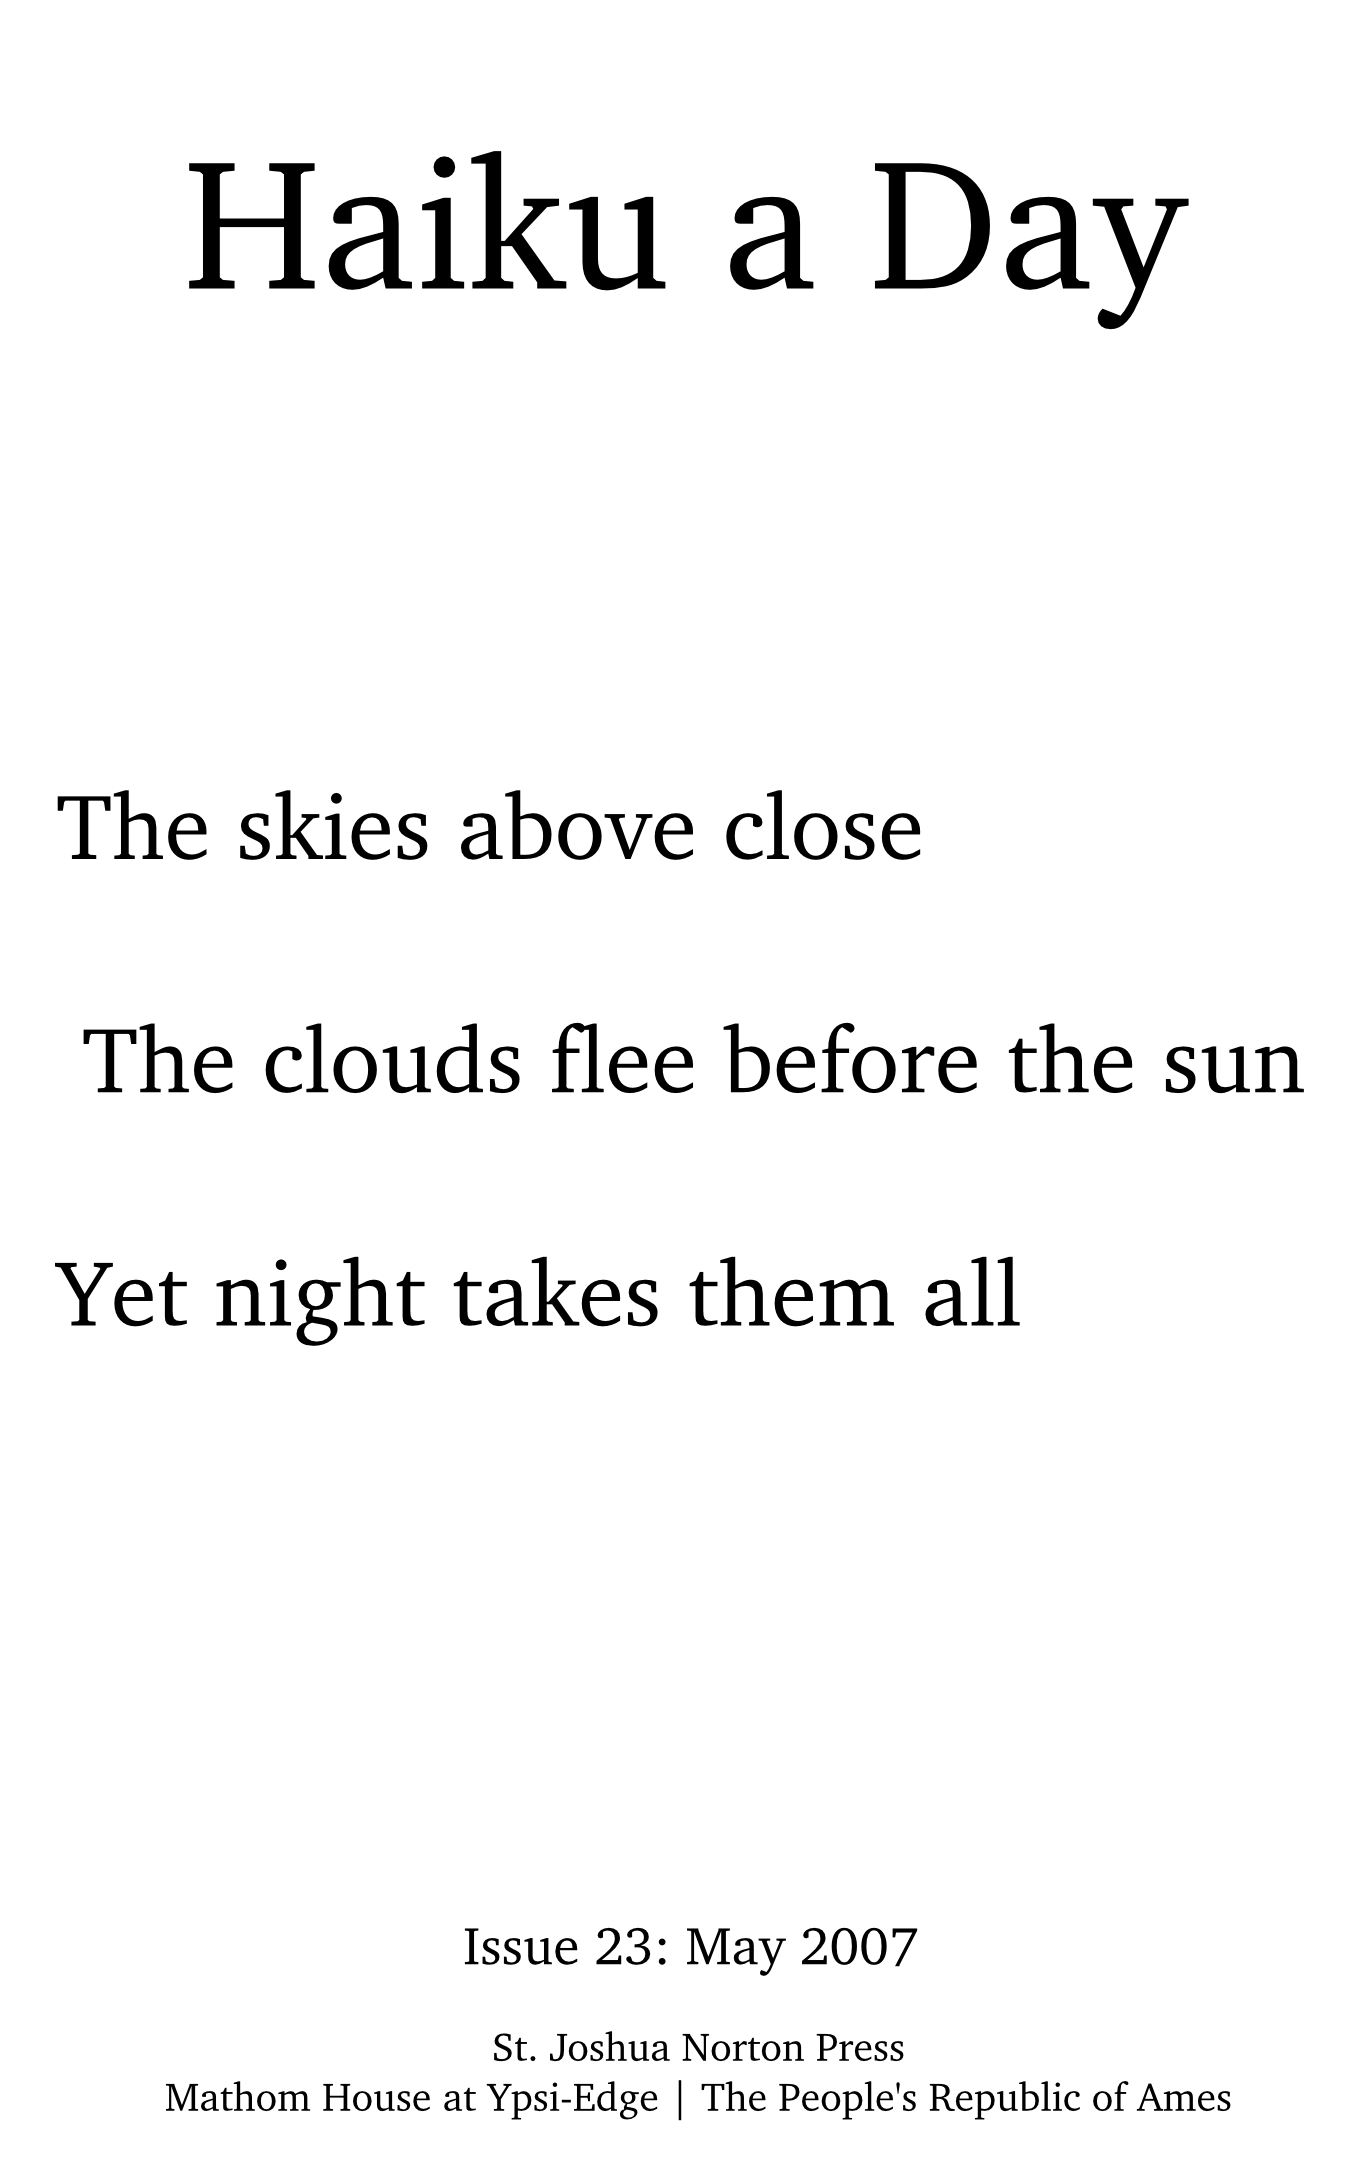
\includegraphics{frontpage.png}

\newpage

The summer continues and Ypsilanti is a beautiful place. 
Nice parks and neat neighborhoods to walk through, a good
coffee shop to hang out in, interesting things going on.

What more could anyone want?

--- Thomas

http://kula.tproa.net/had/ \\
kula@tproa.net

Download this and previous HADs at the website, so you can
print out you own (DIY, yeah!) or if you want me to send
you one, send me your address, and maybe a stamp if you
are feeling nice. Or send me something you've made ---
trades always appreciated.

1 May 2007

Throw off your shackles! \\
Workers of the world, unite! \\
Or something like that

2 May 2007

``The RAID caught fire'' \\
I didn't do it, I swear \\
It's pretty cool, though

3 May 2007

The nail makes a stand \\
Where wood is rotting away \\
Yet rust may still win

4 May 2007

Give a talk next week \\
Perhaps I should finish it \\
For this, I need tea.


\newpage

5 May 2007

A2 Alleycat \\
I ride over to help out \\
A grand day outside

6 May 2007

Oh no, a sock hole \\
The toes will make their escape \\
Heels will be revealed

7 May 2007

The pencil slashes \\
Making a note that dashes \\
The hope of millions

8 May 2007

Ethiopian \\
Food tasted for the first time \\
Mmm, gomen kitfo 

9 May 2007

A thousand dollar \\
Dinner bill at Oak City \\
I had Mac and Cheese

10 May 2007

S \& E Left Coast \\
I finally meet people \\
I've talked to for years

11 May 2007

Plates of crepes dancing \\
In the city the sun shines \\
Filling me with light


\newpage

12 May 2007

Cities travel by \\
Sparkles of light in the night \\
A bump, and I'm home

13 May 2007

My car dead again \\
Maybe I should let it rot \\
And give up driving

14 May 2007

Grainy bus vision \\
Advertising makes sight bleak \\
On the bus ride home

15 May 2007

New Giants album \\
The first part is a bit slow \\
But the end kicks ass

16 May 2007

Morning tea leaves foam \\
On the inside of the press \\
Abstract sea portrait

17 May 2007

A blog visitor \\
Dinner and conversation \\
Must do it again

18 May 2007

The light at the end \\
Of the trail is a cop car. \\
We pass in the night.

\newpage

19 May 2007

I'm out of Britcoms \\
I'll have to wait for some more \\
Are you free, Netflix?

20 May 2007

Nearly six months here \\
Bedrooms still full of boxes \\
I must unpack books.

21 May 2007

The leafblower can. \\
Who can make some awful noise? \\
The leafblower can.

22 May 2007

Presently the moon \\
Rises over the dark land \\
Casting silver rays

23 May 2007

A harsh wail cries out \\
And screaming, racing away \\
Goes the ambulance

24 May 2007 

Soft pillow beckons \\
Calling me to deep slumber \\
Whispering sweet dreams

25 May 2007

Skittering away \\
A spilt newspaper escapes \\
Breeze bringing freedom


\newpage

26 May 2007

A box spills over \\
Books fall, crushing my poor toe \\
I spit out an oath

27 May 2007

The couch whispering \\
"A nap would be so nice now" \\
I nod, and agree

28 May 2007

Ducks playing downstream \\
While geese look on placidly \\
At Riverside Park

29 May 2007

Sweep the counter clean \\
Make room for new groceries \\
Then put them away

30 May 2007

The alternator \\
Coils spinning in their fields \\
Electricity

31 May 2007

Leafy green treetops \\
Poking above the bus stop  \\
Shading the riders


\newpage


\includegraphics{back.png}

\newpage


\includegraphics{backpage.png}

\end{document}




